\section{Limiti}
\subsection{Introduzione al concetto di limite}

Data\marginnote{11 ott 2021} una funzione $ f:D\to \R $, con $ D \subseteq \R^{n} $ e $ x_0 \in \R^{n} $, ci poniamo l'obiettivo di descrivere il comportamento della funzione quando $ x $ si "avvicina" a $ x_0 $.

Indichiamo con $ x\to x_0 $: "avvicinarsi a $ x_0 $", "essere nei pressi di $ x_0 $". In alcuni casi è intuitivo.
\begin{itemize}
    \item caso 1: \begin{align*}
    f:\R & \to \R \\
    x & \mapsto x^{2}
    \end{align*}\begin{align*}
        x=2 \,&\implies\, f(x)=4 & x\to 2\quad &f(x) \to 4\\
        x=3 \,&\implies\, f(x)=9 & x\to 3\quad &f(x) \to 9\\
        x=-1 \,&\implies\, f(x)=1 & x\to -1\quad &f(x) \to 1
    \end{align*}

    Dobbiamo comunque chiarirlo in termini rigorosi.
    \item caso 2: $ f(t)$ rappresenta un impulso luminoso istantaneo al tempo $ t=2 $
    \begin{center}
        \begin{tikzpicture}
            \begin{axis}[
                xlabel=$t$,
                ylabel=$y$,
                axis equal,
                axis lines=middle,
                enlargelimits,
                xmax=5,
                xmin=0,
                ymax=4,
                ymin=-1,
                xtick={2},
                ytick={3},
                scale only axis, 
                height=4cm, 
                width=4cm
                ]
            \addplot [blue, no marks, thick] coordinates {(0,0) (7,0)};
            \addplot [white, thick, only marks] coordinates {(2,0)};
            \addplot [blue, thick, only marks] coordinates {(2,3)};
            \addplot [blue, thick, mark=o] coordinates {(2,0)};
            \end{axis}
        \end{tikzpicture}
    \end{center} dove \[
        f(t)=\begin{cases}
            0 & t\neq 2\\
            3 & t=2
        \end{cases}
    \]
    Se $ t $ si avvicina a $ 2 $, $ f(t) $ a cosa si avvicina? \[
        t\to 5 \qquad f(t)\to ?
    \]
    \item Sia $ f $ tale che \begin{align*}
    f: \N & \to \R \\
    n & \mapsto \frac{1}{n!}
    \end{align*} dove \[
        n!=\begin{cases}
            n(n-1)(n-2) \cdot \cdots \cdot 2 \cdot 1 &n \in \N\setminus\{0\}\\
            1 &n =0
        \end{cases}
    \]
    \[
        f(3)=\frac{1}{3!}=\frac{1}{6}
    \] ma se $ n\to 3 $ cosa vuol dire $ f(n)\to $?

    Per $ n $ che diventa ``molto grande'', $ f(n) $ si ``avvicina a 0''.
\end{itemize}
Per chiarire i concetti di \begin{itemize}
    \item $ x\to x_0 $ utilizzeremo gli intorni $ U(x_0) $ (Topologia in $ \R^{n} $);
    \item $ f(x)\to l \in \R $ utilizzeremo gli intorni $ U(l) $ (Topologia in $ \R $)
    \item Per chiarire se $ x $ può avvicinarsi a $ x_0 $ useremo il concetto di \textit{punto di accumulazione};
    \item Per chiarire il concetto di $ x $ ``grande'', $ f(x) $ ``grande'' dobbiamo estendere la retta $ \R $ dei numeri reali.
\end{itemize}

\subsection{Estensione di $ \R $}
\definizione{}{
    Dati i simboli $ + \infty $, $ - \infty $ diciamo \textit{retta reale ampliata} (estesa) l'insieme \begin{equation}
        \R^{*}:= \R \cup\{+ \infty, - \infty\}
    \end{equation}
}

In $ R^{*} $ possiamo introdurre una relazione di ordine ($\le$)\begin{itemize}
    \item $ x, y \in \R \subseteq \R^{*} $: $ x\le y $ come usuale
    \item $ \forall\, x \in \R^{*} $: $ - \infty \le x \le + \infty $
\end{itemize}
Si verifica che $ \le $ è di ordine totale in $ \R^{*} $: $ \R^{*} $ è insieme totalmente ordinato.

Non è possibile introdurre in $ \R^{*} $ una struttura algebrica che soddisfi gli assiomi $ \mathcal{R}_1 $, $ \mathcal{R}_2 $, $\mathcal{R}_3$.

\attenzione{$\R^{*}$ non è un campo, e $ + \infty $, $ - \infty $ non sono numeri.}

Introduciamo in $ \R^{*} $ una struttura topologica tramite la definizione di intorno per $ x_0 \in \R^{*} $.
Se $ x_0 \in \R $ diciamo intorno di $ x_0 $, $ U(x_0) $ tale che $ \exists\, r>0 $ tale per cui $ B_{r}(x_0) \subseteq U(x_0)  $.

Diciamo \textit{intorno di } $ + \infty $ di ampiezza $ a>0 $ \[
    I_{a}(+ \infty)=U(+ \infty)=\{x \in \R^{*}\,|\, a < x \le + \infty\} 
\]

Diciamo \textit{intorno di } $ - \infty $ di ampiezza $ a>0 $ \[
    I_{a}(- \infty)=U(- \infty)=\{x \in \R^{*}\,|\, - \infty \le x <a\} 
\]

Osserviamo che \[
    x_0 \in U(x_0); \qquad + \infty \in U (+ \infty); \qquad - \infty \in U(- \infty)
\]

\rule{7em}{.4pt}

Possiamo costruire una corrispondenza biunivoca tra \[\R^{*}\longleftrightarrow [-1, 1]=\{x \in \R\,|\, -1\le x\le 1\}\]
\begin{center}
    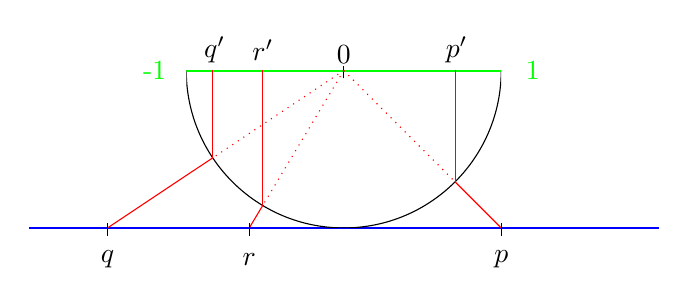
\begin{tikzpicture}[scale=2]
        \draw [blue, thick] (-2, 0) -- (2, 0);
        \begin{scope}
            \clip (-1, 0) rectangle (1,1);
            \draw (0,1) circle (1);
            \draw [green, thick] (-1, 1) -- (1,1);
        \end{scope}
        \node at (-1.2, 1) {\textcolor{green}{-1}};
        \node at (1.2, 1) {\textcolor{green}{1}};
        \node at (0, 1.1) {0};
        \draw (0, 0.95) -- (0, 1.03);
        \draw [red] (0.707, 0.293) -- (1, 0);
        \draw [red, dotted] (0, 1) -- (0.707, 0.293);
        \draw (1, -0.05) -- (1, 0.03);
        \draw [red] (0.707, 0.293) -- (0.707, 1);%
%
    \draw [red] (-0.832, 0.445) -- (-1.5, 0);
    \draw [red, dotted] (0, 1) -- (-0.832, 0.445);
    \draw (-1.5, -0.05) -- (-1.5, 0.03);
    \draw [red] (-0.832, 0.445) -- (-0.832, 1);%
%
    \draw [red] (-0.514, 0.143) -- (-0.6, 0);
    \draw [red, dotted] (0, 1) -- (-0.514, 0.143);
    \draw (-0.6, -0.05) -- (-0.6, 0.03);
    \draw [red] (-0.514, 0.143) -- (-0.514, 1);%
%
    \node at (-1.5, -0.2) {$q$};
    \node at (1, -0.2) {$p$};
    \node at (-0.6, -0.2) {$r$};
    \node at (-0.82, 1.13) {$q'$};
    \node at (0.717, 1.13) {$p'$};
    \node at (-0.514, 1.13) {$r'$};
    \end{tikzpicture}
\end{center}
\[
    \R\longleftrightarrow (-1, 1)\qquad + \infty \longleftrightarrow 1\qquad - \infty \longleftrightarrow -1.
\]

\paragraph{Estremo superiore (inferiore) in $ \R^{*} $}

Sia $ X \subseteq \R $, $ X $ limitato superiormente (limitato inferiormente) 

$\overset{\mathcal{R}_4}{\implies}$ $ \exists\, \sup X \in \R $ ($\exists\, \inf X \in \R$)

Diciamo che \begin{itemize}
    \item se $ X $ non è limitato superiormente, allora $ \sup X = +\infty $
    \item se $ X $ non è limitato inferiormente, allora $ \inf X = - \infty $
\end{itemize}
Concludiamo che $ \forall\, X \subseteq \R $, $ X $ ammette $ \sup X $ e $ \inf X $ in $ \R^{*} $

\teorema[(di Bolzano Weierstrass in $ \R^{*} $)]{bolzwreinrrstar}{
    Sia $ X \subseteq \R $, $ X $ infinito 
    
    $\implies$ $ X $ ammette almeno un punto di accumulazione in $ \R^{*} $
}
\osservazione{
    $ + \infty $ è punto di accumulazione per $ \N $, ed è l'unico.

    $ + \infty, - \infty $ sono gli unici punti di accumulazione per $ \Z $.
}

\subsection{Estensione di $ \R^{n} $}

Indichiamo \begin{equation}
    \dot{\R}^{n}=\R^{n}\cup\{ \infty\}
\end{equation}

Per quanto riguarda la topologia, diciamo intorno di $ \infty $ di ampiezza $ a>0 $ \[
    I_{a}( \infty)=U( \infty) = \{x \in \R^{n};\,\tc\, |x|>a\}\cup\{\infty\}
\]

Se $ n=1 $, $ \dot{\R}= \R\cup\{\infty\} $ \[
    I_{a}( \infty)=\{x \in \R\:\tc\, x<-a\,\lor\, x>a\}\cup\{\infty\} 
\]
\begin{center}
    \begin{tikzpicture}
        \draw [dashed] (-1, 0) -- (1, 0); 
        \node at (1, 0.25) {$a$};
        \node at (-1, 0.25) {$-a$};
        \node at (0, 0.25) {$0$};
        \draw (0, -0.1) -- (0, 0.03);
        \draw [blue, thick] (1, -0.1) -- (1, 0.03);
        \draw [blue, thick] (-1, -0.1) -- (-1, 0.03);
        \draw [blue, thick] (-4, 0) -- (-1, 0);
        \draw [blue, thick, dashed] (-4, 0) -- (-5, 0);
        \draw [blue, thick] (4, 0) -- (1, 0);
        \draw [blue, thick, dashed] (4, 0) -- (5, 0);
    \end{tikzpicture}
\end{center}

\proprieta{}{
    È possibile mettere in corrispondenza biunivoca $ \dot{\R} $ e la circonferenza $ C_{1}(0)  $ (di centro 0 e raggio 1):
    \begin{center}
        \begin{tikzpicture}
            \draw (-5,0) -- (5,0);
            \draw (0,1) circle (1);
            \node at (0, 2.3) {\textcolor{green}{$P$}};
            \fill [green] (0,2) circle (0.05);
            \draw [red] (3,0) -- (0,2);
            \fill [blue] (3,0) circle (0.05);
            \node at (3, 0.3) {\textcolor{blue}{$x$}};
            \node at (1.15,1.645) {\textcolor{green}{$x'$}};
            \fill [green] (0.923,1.385) circle (0.05);
        \end{tikzpicture}
    \end{center}
    \[
        P\longleftrightarrow \infty\qquad \begin{aligned}
            x'&\longleftrightarrow x\\
            C_{r}(0)\setminus \{P\}&\longleftrightarrow \R 
        \end{aligned}
    \]
}

\osservazione{
    Dato $ x_0 \in \R^{n} $ indichiamo con \[
        \dot{U}_r(x_0)=U_{r}(x_0)\setminus \{x_0\} 
    \] In particolare \[
        \dot{B}_r(x_0)=B_{r}(x_0)\setminus\{x_0\} 
    \]
    \begin{align*}
        \dot{I}_{a}( \infty) &= I_{a}( \infty)\setminus\{ \infty\} \\
        \dot{I}_{a}(+ \infty) &= I_{a}( +\infty)\setminus\{ +\infty\}=(a, + \infty)=\{x \in \R;\, x>a\}\\
        \dot{I}_{a}(- \infty) &= I_{a}( -\infty)\setminus\{ -\infty\}=(-\infty, -1)=\{x \in \R;\, x<-a\}
    \end{align*}

    Distingueremo sempre $ \dot{I}(x_0) $ da $ I(x_0) $, con $ x_0 \in \R $, mentre spesso scriveremo \[
        I_{a}( \infty)\qquad I_{a}(+ \infty)\qquad I_{a}(- \infty)   
    \] in luogo di \[
        \dot{I}_{a}( \infty)\qquad \dot{I}_{a}(+ \infty)\qquad \dot{I}_{a}(- \infty)   
    \]
}

\subsection{Limite di una funzione}

Data $ f:\R\to \R $ (a valori reali)
\definizione{}{
    Data \begin{align*}
    f:D & \to \R \\
    x & \mapsto f(x)
    \end{align*} $ D=\dom f \subseteq \R $, consideriamo $ x_0 \in \R^{*} $, $ x_0 $ punto di accumulazione del dominio $ D $ ($ x_0 \in D'$), dato $ l \in \R^{*} $, diciamo che $ l $ è il limite di $ f $ per $ x $ che tende a $ x_0 $.

    Scriviamo \begin{equation}
        l= \lim_{x\to x_0} f(x)
    \end{equation} equivalentemente \[
        \Bigl(f(x) \xrightarrow[x\to x_0]{} l;\qquad f(x)\to l\quad x\to x_0\Bigr)
    \] se \begin{equation}
        \forall\, V(l)\quad \exists\, U(x_0)\,\tc\quad x \in (U\cap D)\setminus\{x_0\} \,\implies\, f(x) \in V(l)
    \end{equation} con $ V(l) $ intorno di $ l $ e $ U(x_0) $ intorno di $ x_0 $.
}

Schematizzando \begin{enumerate}
    \item [\textcolor{green}{1.}] Consideriamo un generico intorno di $ l $ ($ \forall\,V(l)$);
    \item [\textcolor{red}{2.}] cerchiamo un intorno di $ x_0 $ opportuno ($\exists\, U(x_0)$): $ U(x_0) $ dipenderà dalla scelta di $ V(l) $;
    \item [\textcolor{blue}{3.}] verifichiamo che $ \forall\, x \in U(x_0) \,\land\, x \in D\,\land\, x \neq x_0 $ si abbia $ f(x) \in V(l) $.
\end{enumerate}

Verificati 1. 2. 3. possiamo dire che \[
    \lim_{x\to x_0} f(x) =l
\]

\osservazione{
    \begin{itemize}
        \item $ x_0 $ è di accumulazione per $ D $, è possibile che $ x_0\notin D $, ossia è possibile che $ f(x_0)=\nexists $;
        \item nel caso in cui $ x_0 \in D $ allora $ f(x_0) $ esiste, ma non è detto che $ f(x_0) $ coincida con il limite $ l $.
    \end{itemize}
    Noi verifichiamo che $ f(x) \in V(l) $ solo per $ x \in U(x_0)\,\land\, x \neq x_0 $. Potrebbe verificarsi $ f(x_0)\notin V(l) $

    Nel verificare che $ \displaystyle \lim_{x\to x_0} f(x) =l $ il comportamento di $ f $ nel punto $ x_0 $ è ininfluente.
}

\rule{7em}{.4pt}

Decliniamo la definizione di limite \[
    \lim_{x\to x_0} f(x) =l\qquad x_0 \in \R^{*}, l \in \R^{*}
\] nei vari casi: \[
    x_0 \in \R; \quad x_0=\pm \infty;\quad l \in \R;\quad l =\pm \infty
\]

\underline{Caso 1}: $ x_0 \in \R $, $ l \in \R $, $ x_0 $ di accumulazione per $ D=\dom f$: \[
    \lim_{x\to x_0} f(x) =l
\]
\[
    \forall\, \parentesi{(l- \varepsilon,\, l+ \varepsilon)}{V(l)}\quad \exists\, \parentesi{(x_0-\delta,\, x_0+\delta)}{U(x_0)}\,\tc\quad \parentesi{0<|x-x_0|<\delta}{x \in U\,\land\, x \neq x_0}\,\land\, x \in D \,\implies\, \parentesi{|f(x)-l|< \varepsilon}{f(x) \in V(l)}
\] Perciò \[
    \forall\,V(l) \longleftrightarrow \forall\, \varepsilon>0\qquad \exists\, U(x_0)\longleftrightarrow \exists\, \delta>0
\] Allora \[
    \lim_{x\to x_0} f(x) =l
\] se \begin{equation}
    \forall\, \varepsilon>0\quad \exists\, \delta>0\,\tc\quad 0<|x-x_0|<\delta\,\land\, (x \in D) \,\implies\, |f(x)-l|< \varepsilon
\end{equation}

\underline{Caso 2}: $ x_0 \in \R $, $ l = + \infty $, $ x_0 $ di accumulazione per $ D=\dom f$: \[
    \lim_{x\to x_0} f(x) = + \infty
\]
\[
    \forall\, \parentesi{(M,\, + \infty)}{V(l)}\quad \exists\, \parentesi{(x_0-\delta,\, x_0+\delta)}{U(x_0)}\,\tc\quad \parentesi{0<|x-x_0|<\delta}{x \in U\,\land\, x \neq x_0}\,\land\, x \in D \,\implies\, \parentesi{f(x)>M}{f(x) \in V(l)}
\] Perciò \[
    \forall\,V(l) \longleftrightarrow \forall\, M>0
\] Allora \[
    \lim_{x\to x_0} f(x) =+ \infty
\] se \begin{equation}
    \forall\, M>0\quad \exists\, \delta>0\,\tc\quad 0<|x-x_0|<\delta\,\land\, (x \in D) \,\implies\, f(x)>M
\end{equation}

In più
\[\displaystyle \lim_{x\to x_0} f(x) =- \infty\] se \begin{equation}
    \forall\, M>0\quad \exists\, \delta>0\,\tc\quad 0<|x-x_0|< \delta \,\land\, x \in D \,\implies\, f(x)<-M
\end{equation}

Così via per gli altri casi

\underline{Caso} $ l= \infty \in \dot{\R} $, $ x_0 \in \R $.
\[
    \forall\, \parentesi{x<-M\,\lor\,x>M}{V(l)}\quad \exists\, U(x_0)\,\tc\quad x \in U\,\land\, x \neq x_0\,\land\, x \in D \,\implies\, \parentesi{f(x)<-M\,\lor\,f(x)>M}{f(x) \in V(l)}
    \] Perciò \[
        \forall\,V(l) \longleftrightarrow \forall\, M>0
    \]Allora \[
        \lim_{x\to x_0} f(x) = \infty
    \] se\begin{equation}
        \forall\,M>0\quad \exists\, \delta>0\,\tc\quad 0<|x-x_0|<\delta\,\land\, x \in D \,\implies\, f(x)<-M\,\lor\, f(x)>M
    \end{equation}

\esempio{
    Verifichiamo che \[
        \lim_{x\to 0} \sin x=0
    \] ossia \[
        \forall\, \varepsilon>0\quad \exists\, \delta>0\,\tc\quad 0<|x|< \delta \,\implies\,|\sin x|< \varepsilon
    \]

    Osserviamo che per $ -\frac{\pi}{2}< x<\frac{ \pi}{2} $, $ -x<\sin x < x $, ossia \begin{equation*}
        |x|<\frac{ \pi}{2} \,\implies\,|\sin x|<|x|
    \end{equation*} Consideriamo $ d\le \frac{\pi}{2} $ \begin{equation*}
        |x|<\delta \,\implies\,|\sin x|<|x|<\delta
    \end{equation*}

    Sia $ \delta =\min \bigl\{\frac{\pi}{2}, \varepsilon\bigr\} $ allora \[
        |\sin x|<|x|<\delta \le \varepsilon
    \] dunque abbiamo verificato che \[
        \forall\, \varepsilon>0\quad \exists\, \delta =\min\bigl\{ \varepsilon, \frac{\pi}{2}\bigr\}\,\tc\quad 0<|x|<\delta \,\implies\, |\sin x| < \varepsilon
    \]
}

\esempio{
    Verifichiamo che \[
        \lim_{x\to 2} x^{2} =4
    \] ossia \[
        \forall\, \varepsilon>0\quad \exists\, \delta>0\,\tc\quad 0<|x-2|< \delta \,\implies\, |f(x)-4|< \varepsilon
    \]

    \[
        |f(x)-4|< \varepsilon\,\iff\, |x^{2}-4|< \varepsilon \,\iff\, |x-2|\,|x+2|< \varepsilon
    \] Consideriamo $ \delta \le 1 $ allora $ |x-2|<1 $ osssia $ 1<x<3 $, allora $ 3 \le x+2 \le 5 $. Allora per $ \delta <1 $ si avrà per ogni $ |x-2|<\delta $ \[
        |x-2|\,|x+2|\le 5 |x-2|
    \] Allora, se \[
        5\,|x-2|< \varepsilon \,\implies\, |x^{2}-4|=|x-2|\,|x+2|< \varepsilon
    \] allora, preso \[
        \delta =\min\biggl\{1, \frac{ \varepsilon}{5}\biggr\}
    \] si ha \[
        |x-2|<\delta \,\implies\,|x^{2}-4|< \varepsilon
    \]

    Dunque abbiamo verificato che 
    \[
        \forall\, \varepsilon>0\quad \exists\, \delta>0\,\tc\quad 0<|x-2|< \delta \,\implies\, |f(x)-4|< \varepsilon
    \] ossia 
    \[
        \lim_{x\to 2} x^{2} =4
    \]
}